\documentclass[10pt,a4paper]{article}
\usepackage[utf8]{inputenc}
\usepackage[english]{babel}
\usepackage[T1]{fontenc}
\usepackage{amsmath}
\usepackage{amsfonts}
\usepackage{amssymb}
\usepackage{subcaption}
\usepackage{makeidx}
\usepackage{graphicx}
\usepackage{fourier}
\usepackage{listings}
\usepackage{color}
\usepackage{hyperref}
\usepackage[left=2cm,right=2cm,top=2cm,bottom=2cm]{geometry}
\author{Tommy Müller, Marcus Dittrich, Vincent Noculak}
\title{Rastertunnelmikroskop}

\lstset{language=C++,
	keywordstyle=\bfseries\color{blue},
	commentstyle=\itshape\color{red},
	stringstyle=\color{green},
	identifierstyle=\bfseries,
	frame=single}
\begin{document}

\maketitle
\newpage
\tableofcontents
\newpage

\section{Vermessung von Graphit }

\subsection{ Kantenhöhen}

Mit dem Rastertunnelmikroskop haben wir 79 Bilder gemacht. Davon waren 16 zum Kantenvermessen geeignet.
Diese Bilder haben wir mit dem Tool WSxM 4.0 Beta 8.2 vermessen. 
Die Funktion "Local plane" und "profile" nutzen wir bei den Bildern. "Local plane" reskaliert, nach Auswahl von ebenen Flächen, das gesamte Bild.  Die Funktion "profile" lieferte ein Höhenprofil zwischen zwei ausgewählten Punkten. (Siehe Bilder der Kanten unten)
Viele Bilder waren fehlerhaft und konnten nicht zur Bestimmung von Kantenhöhen verwendet werden. Unter anderem waren thermische Verschiebung (Drift), Creep und Bildfehler  \ref{b12} das Hauptproblem oder keine verwertbare Kante auf Bildern. Wir haben jede Kante an 5 unterschiedlichen Orten vermessen, dies lieferte den Mittelwert und den Fehler als Standardabweichung.



\subsection{Beispiel Kanten}

\begin{figure}[]
	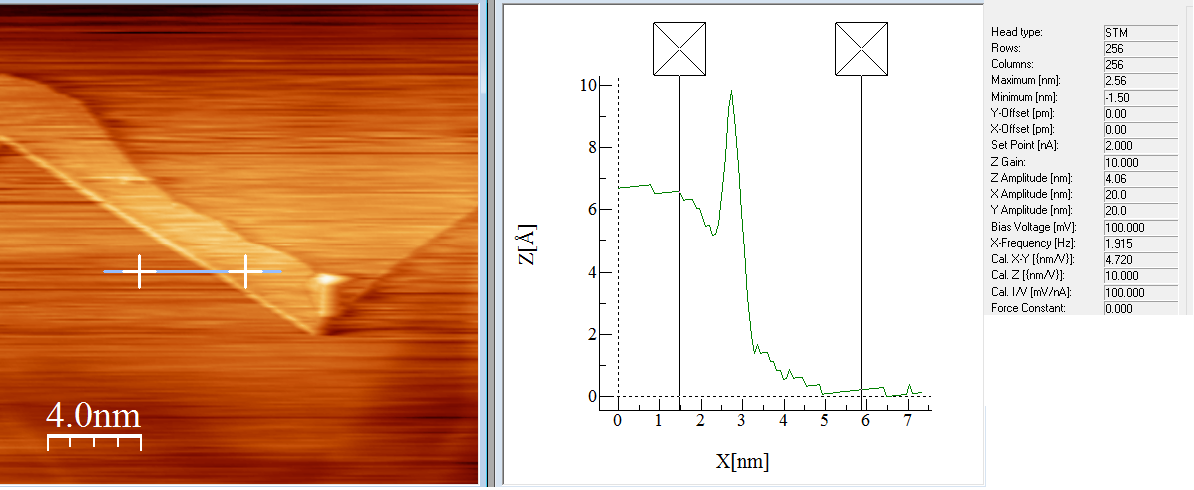
\includegraphics[scale = 0.3]{bild00.png}
	\centering
	\caption{Bild 0. Kante 0.637 nm und RTM Daten}
	\label{b0}
\end{figure}

\begin{figure}[]
	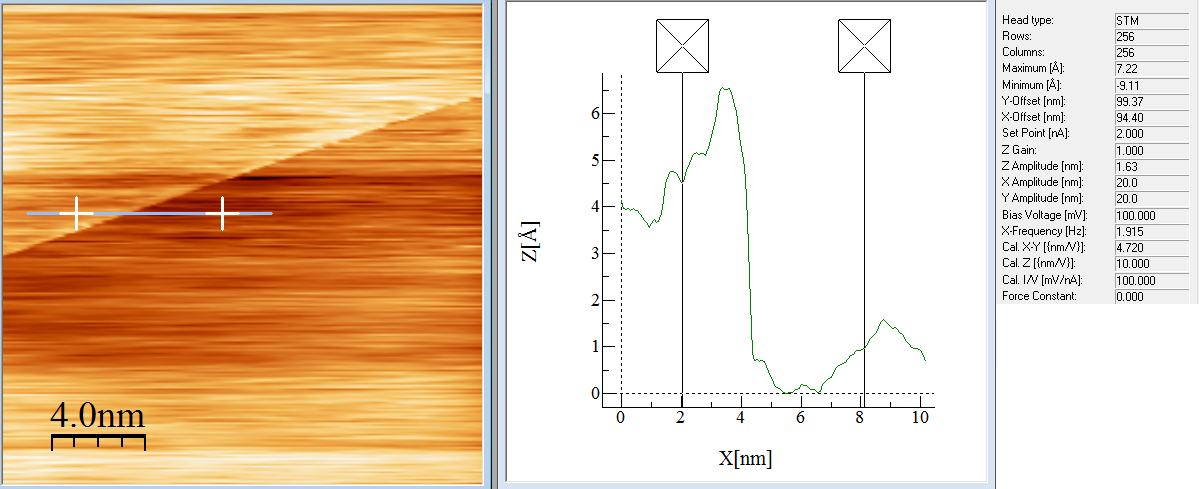
\includegraphics[scale = 0.3]{bild11.png}
	\centering
	\caption{Bild 11. Kante 0.353 nm und RTM Daten}
	\label{b11}
\end{figure}
\begin{figure}[]
	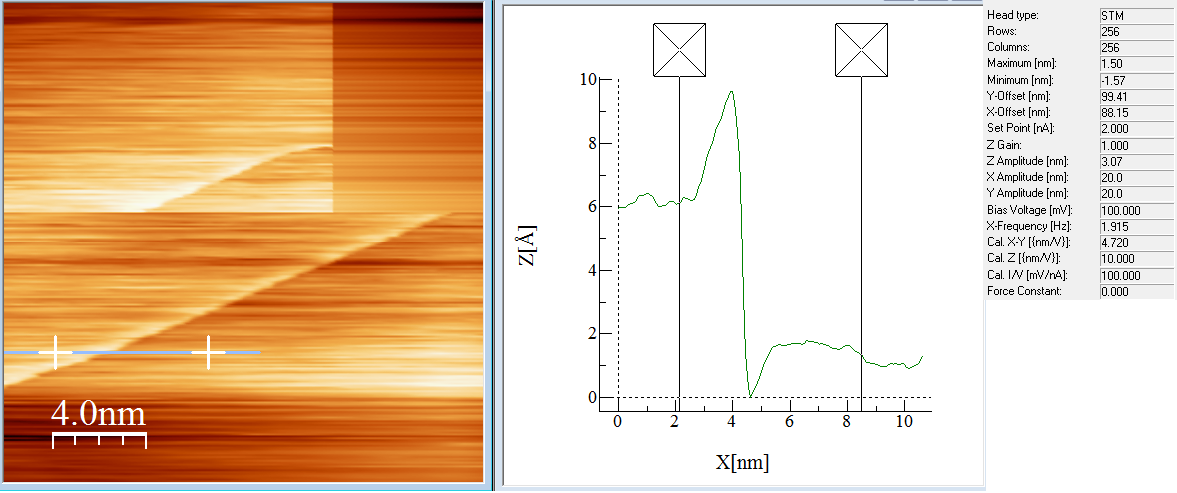
\includegraphics[scale = 0.3]{bild12.png}
	\centering
	\caption{Bild 12. Kante 0.447 nm und RTM Daten}
	\label{b12}
\end{figure}




In dem Diagramm \ref{kantendia} sind alle gemittelten Kanten eingetragen Die Höhen gingen von 0.272  $ \pm 0.149 $ nm bis 1.893 $ \pm 0.250 $ nm. Im Folgenden haben wir die Höhen in einem Diagramm\ref{kantendia} aufgetragen und die theoretischen Kanten mit den roten Linien markiert.

\begin{figure}[]
	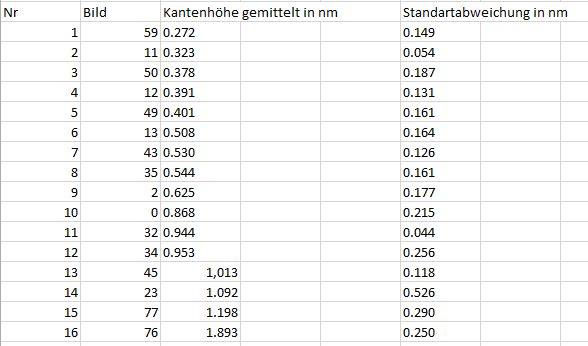
\includegraphics[scale = 0.5]{Kantengeordnetrichtig.png}
	\centering
	\caption{Liste der ordeneten Kanten}
	\label{list}
\end{figure}

\begin{figure}[]
	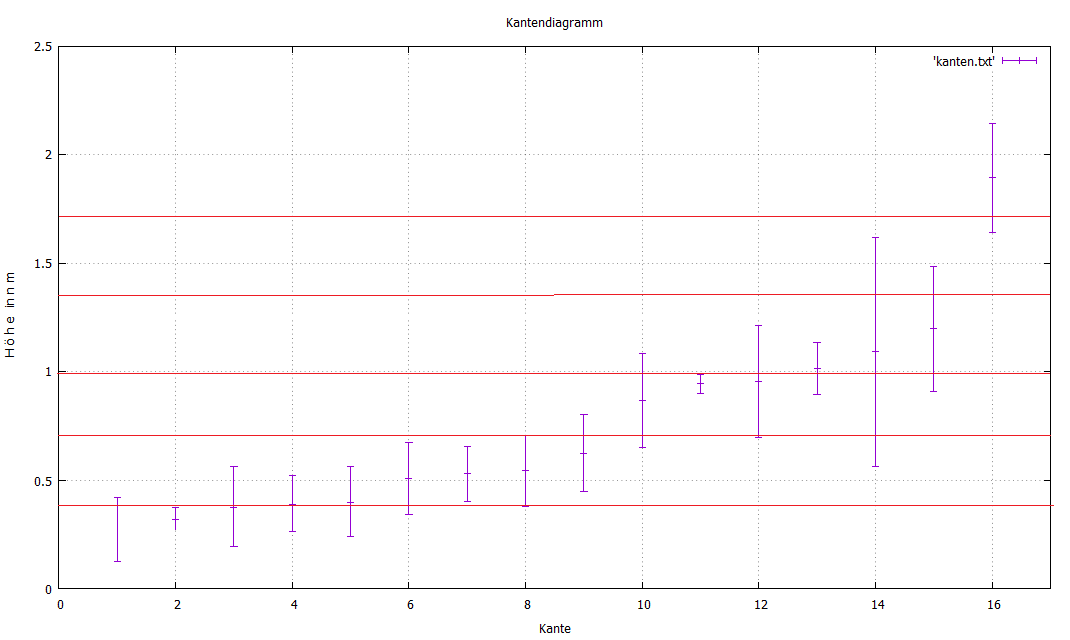
\includegraphics[scale = 0.5]{kantendia.png}
	\centering
	\caption{Diagramm Höhe der Kanten sowie in Rot Theoretische Kantenhöhen}
	\label{kantendia}
\end{figure}

In dem Diagramm zu den Höhen sehen wir eine Ansammlung von Kanten bei den N = 1 und 3 diese Kanten werden am besten durch unsere Messungen repräsentiert. Die anderen theoretischen Kanten werden nur bedingt durch unsere Messergebnisse wiedergespiegelt.
Den Z Gain konnten wir leider nicht ermitteln da wir weder die Länge des Piezo Elementes hatten noch die  piezoelektrische Konstante der Spitze.



\subsection{ Diskussion}

Beim Vergleichen der theoretischen Kanten mit dem Messergebissen muss drauf geachtet werden das die Kanten nicht durch Drift oder Creep unscharf werden bzw keine Kanten im Kristall sind. Die Form der Spitze ist entscheidend, da diese aber mit einer Drahtschere gefertigt wurden(keine einatomige Spitze), sind Messfehler zu erwarten. 
Das vermessen der Bilder ergab leider nur 16 Kanten. Diese Kanten sind nach der Höhe geordnet und im Diagramm \ref{kantendia} zu sehen. Wir konnten mit unseren Messergebnissen die theoretischen Kanten relativ gut darstellen. Vor allem den ersten und dritten Netzebenenabstand können unsere Messergebnisse rekonstruieren. Einige Messergebisse sind fast genau zwischen zwei Ebenen, dies könnte an der schlechte Wahl von Messpunkten am Bild liegen. Eine vorab Sondierung der Bilder wäre von Nöten gewesen mehr Kanten zu erfasst und die Ergebnisse klarer zu gestalten.

\end{document}